\section{Data Reduction}
% description of how reduced and calibrated  your data

In this session we discuss how we treat the raw data, which was registered with the  software LoggerPro \cite{loggerpro} as measurements of the total output voltage vs time of  signal.

\subsection{Treatment of the Voltage V(t) Raw Data}

To normalize and delogarithm  all the four sets of data described in the section \ref{observations},  we use the equations (\ref{pdb}) and (\ref{pdb2}). The negative slope indicates that the output voltage decreases as the input power increase. The interferometry results for the Sun and for the satellite are shown in the figures \ref{voltpow2} and \ref{voltpow3}. The total power is the amplitude squared of the summed  electric vectors of the electromagnetic signals, as we described before.




 \begin{figure}[htb]
\begin{center}
 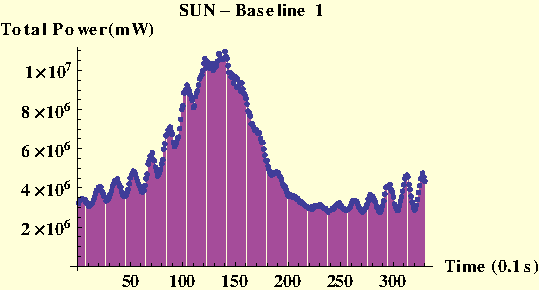
\includegraphics[scale=0.7]{plots/sun1pow.pdf}
 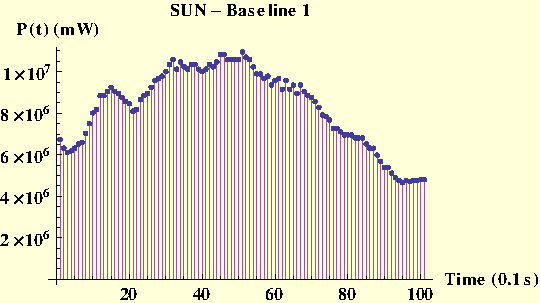
\includegraphics[scale=0.7]{plots/sun1powc.pdf}
 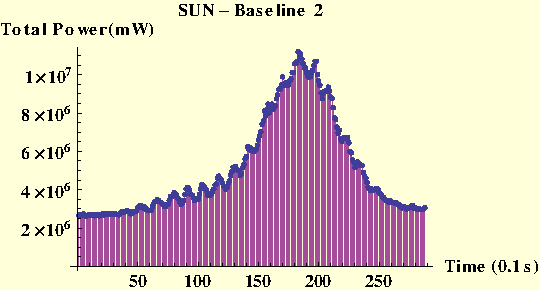
\includegraphics[scale=0.7]{plots/sun2pow.pdf}
 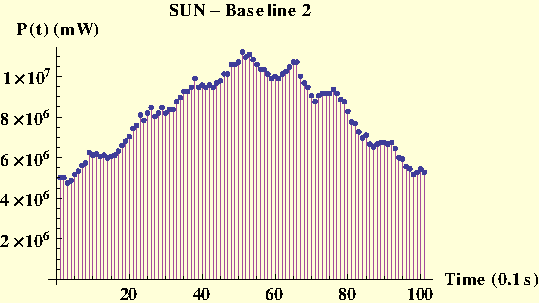
\includegraphics[scale=0.7]{plots/sun2powc.pdf}
 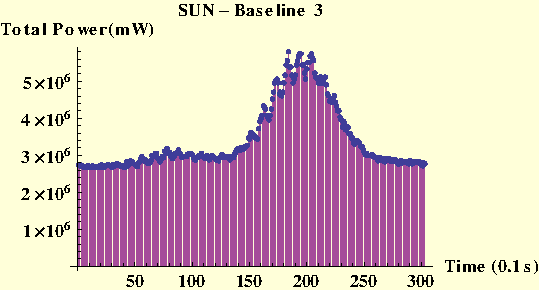
\includegraphics[scale=0.7]{plots/sun3pow.pdf}
 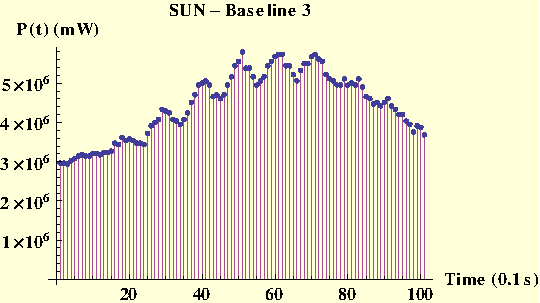
\includegraphics[scale=0.7]{plots/sun3powc.pdf}
 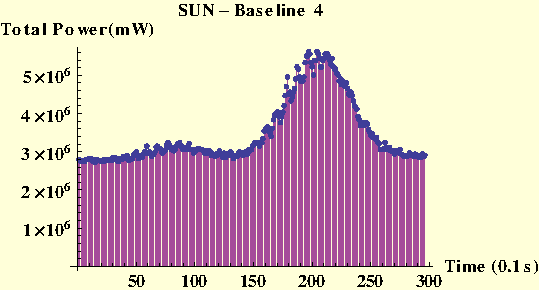
\includegraphics[scale=0.7]{plots/sun4pow.pdf}
 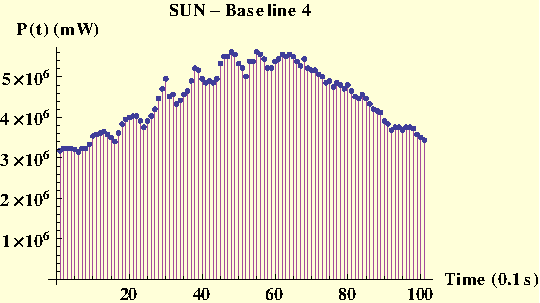
\includegraphics[scale=0.7]{plots/sun4powc.pdf}
 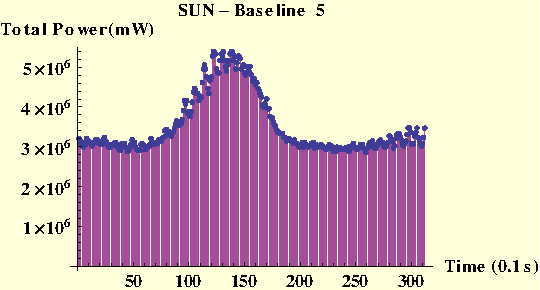
\includegraphics[scale=0.7]{plots/sun5pow.pdf}
 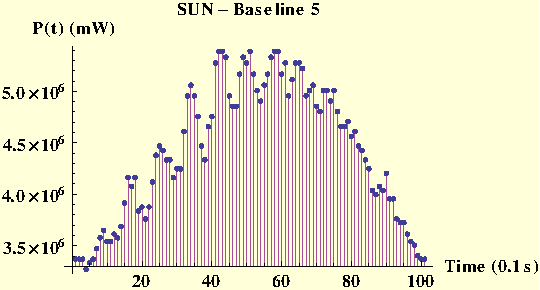
\includegraphics[scale=0.7]{plots/sun5powc.pdf}
\caption{Interferometer measurements of total power of the Sun, in function of time, for the five set of measurements. On the right, after the  cuts.}
\label{voltpow2}
\end{center}
\end{figure}

 \begin{figure}[htb]
\begin{center}
 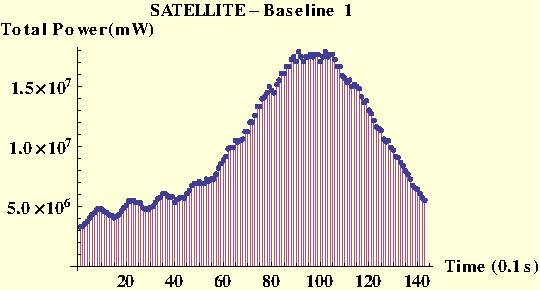
\includegraphics[scale=0.7]{plots/sat1pow.pdf}
 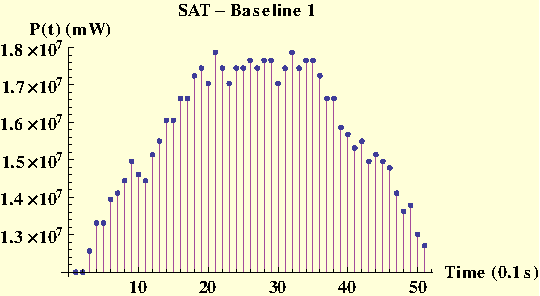
\includegraphics[scale=0.7]{plots/sat1powc.pdf}
 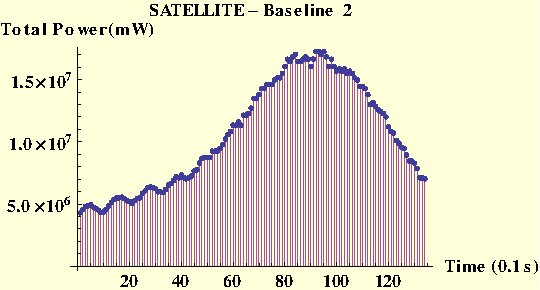
\includegraphics[scale=0.7]{plots/sat2pow.pdf}
 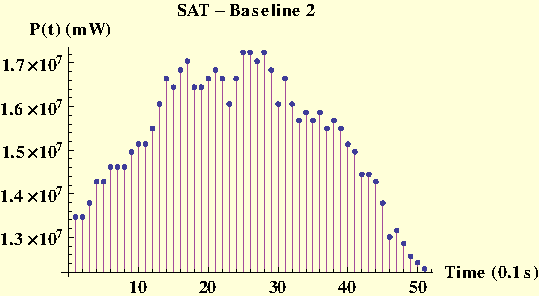
\includegraphics[scale=0.7]{plots/sat2powc.pdf}
 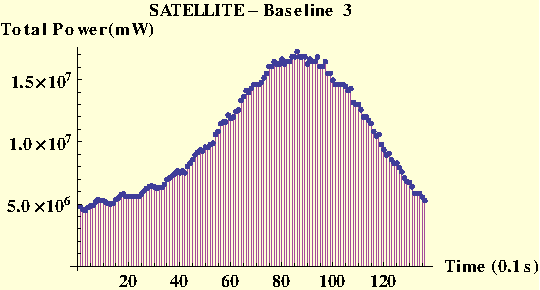
\includegraphics[scale=0.7]{plots/sat3pow.pdf}
 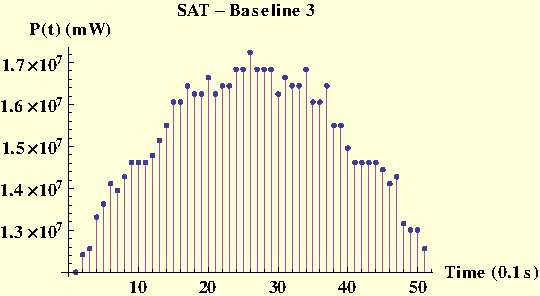
\includegraphics[scale=0.7]{plots/sat3powc.pdf}
 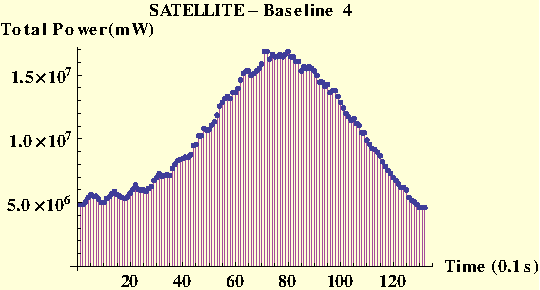
\includegraphics[scale=0.7]{plots/sat4pow.pdf}
 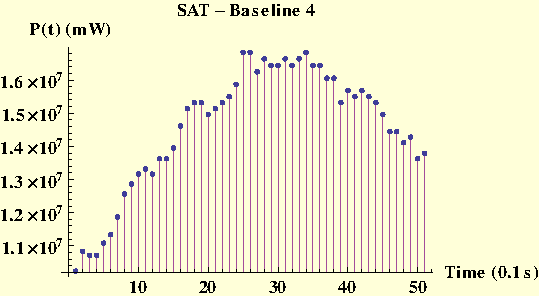
\includegraphics[scale=0.7]{plots/sat4powc.pdf}
 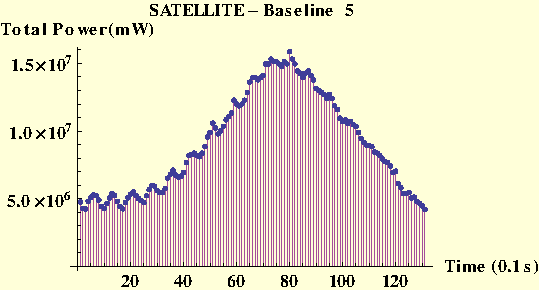
\includegraphics[scale=0.7]{plots/sat5pow.pdf}
 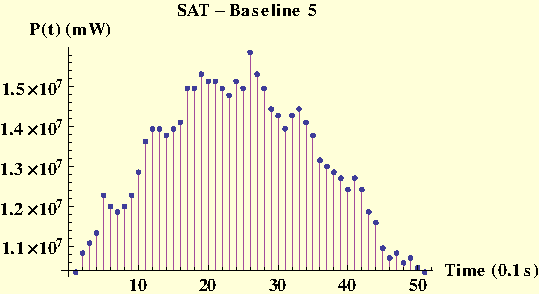
\includegraphics[scale=0.7]{plots/sat5powc.pdf}
\caption{Interferometer measurements of total power of the satellite, in function of time, for the five set of measurements. On the right, after the  cuts.}
\label{voltpow3}
\end{center}
\end{figure}




\bigskip


\subsection{The Single Dish Measurements for the Sun and the Satellite}

In the single dish mode, the size of the solar disk is the {\it deconvolution} of the single dish solar profile with the single dish satellite profile. We report the single dish profile for one of the measurements of each of the sources in the figure \ref{voltpow4}. We use these two profiles to resolve a first approximation of the solar angular diameter.

 \begin{figure}[htb]
\begin{center}
 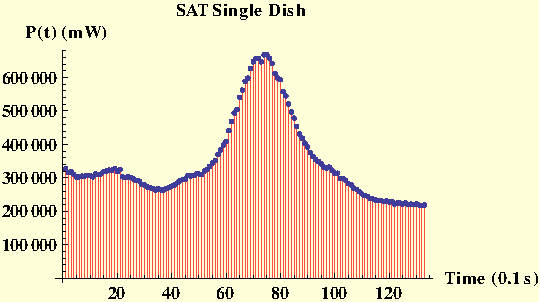
\includegraphics[scale=0.8]{plots/single/1.pdf}
 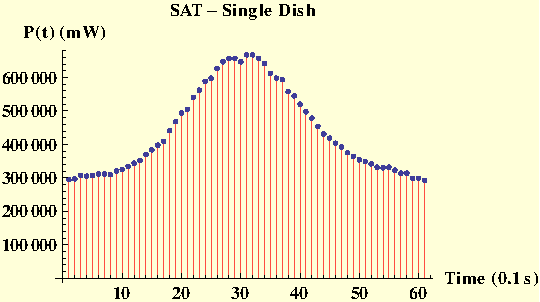
\includegraphics[scale=0.8]{plots/single/2.pdf}
 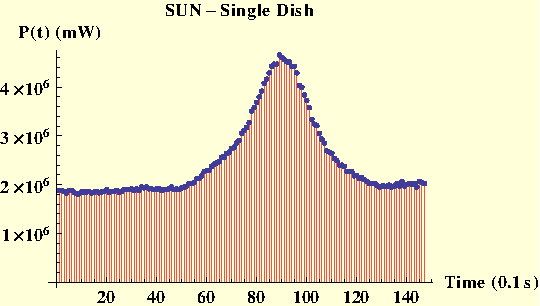
\includegraphics[scale=0.8]{plots/single/3.pdf}
 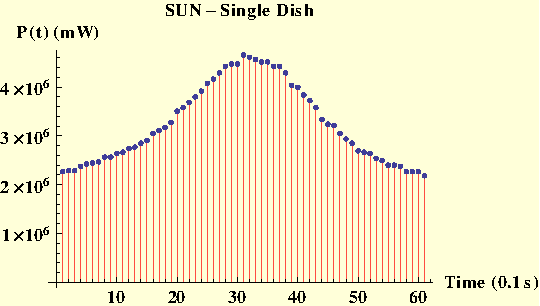
\includegraphics[scale=0.8]{plots/single/4.pdf}

\caption{Single dish measurements for the Sun and the satellite.}
\label{voltpow4}
\end{center}
\end{figure}


